\chapter{Phase I: Analyse}

%Der Software-Entwicklungsprozess gliedert sich in drei Phasen \cite[S. 747]{stroustrup}: 
%\begin{itemize}
	%\item \textbf{Analyse}: Untersuchung der Anforderungen an das System, Eingrenzung des zu l�senden Problems
	%\item \textbf{Design}: Entwurf einer allgemeinen Struktur f�r das System, Beschreibung der Funktionsweise der einzelnen Systemteile
	%\item \textbf{Implementierung}: Umsetzen des Designs in Code, Testen des Systems
%\end{itemize}

%Bei der Entwicklung des \DevEnvs\ wurden die Phasen allerdings nicht in dieser Reihenfolge genau einmal durchlaufen. Das System ist in einem iterativen und inkrementellen Prozess entstanden. Das bedeutet, dass jede Phase mehrmals durchlaufen wurde und zun�chst nur ein kleiner Teil des Systems entwickelt wurde. Nachdem dieser Teil vollst�ndig funktionsf�hig war, wurde mit der Entwicklung des n�chsten Subsystems begonnen. Diesem Vorgehen liegt der \textit{Unified Process} zugrunde; ein h�ufig eingesetzter Prozess zur Entwicklung von Business Anwendungen. Der \textit{Unified Process} empfiehlt, in jeder Phase gewisse Dokumente, Artefakte genannt, zu erstellen. Daf�r wird meistens eine der zahlreichen Diagramm-Arten der \textit{Unified Modelling Language} verwendet. Der \textit{Unified Process} ist jedoch nicht starr, sondern kann an die Komplexit�t und Art des zu entwickelnden Systems angepasst werden. So wurden f�r das \DevEnv\ in der Analyse-Phase ein \textit{Use Case Model} und ein \textit{Domain Model} erstellt.

Bevor mit der eigentlichen Entwicklung des Systems begonnen wurde, mussten zun�chst die Anforderungen an das Tool analysiert werden. Die Anforderungen ergaben sich aus der Betrachtung des Aufbaus und der Funktionsweise von \Horde\ und beziehen die gewonnenen Erfahrungen bei der Entwicklung von \SheepMeUp\ mit ein. Au�erdem mussten die Ziele, die bei der Entwicklung des \DevEnvs\ verfolgt wurden, von bereits vorhandener Software abgegrenzt werden.

In der Analyse-Phase wurden ein \emph{Use Case} Modell und ein Konzeptmodell erstellt, welche die Grundlage f�r die Design-Phase bildeten.

\section{�berblick �ber Horde3D}
Zu Projektbeginn wurde deutlich, dass die Struktur des \DevEnvs\ ma�geblich vom Aufbau und der Funktionsweise von \Horde\ bestimmt wird. Bevor die genauen System-Anforderungen untersucht wurden, wurde ein konzeptuelles Modell von \Horde\ entwickelt. Dabei wurde die interne Repr�sentation der Daten -- also die Klassen und Funktionen, die \Horde\ intern verwendet -- nicht betrachtet. Wichtig ist nur der von au�en festzustellende Aufbau, denn nur davon wird die Struktur des Tools beeinflusst. Da die Dokumentation \cite{h3dmanual} allerdings keine Klassendiagramme enth�lt, musste die Klassenstruktur aus der Beschreibung der API \cite["`Engine API Reference"']{h3dmanual}, der Datenformate \cite["`Data Format Reference"']{h3dmanual} und der Rendering-Pipeline \cite["`Rendering Pipeline Documentation"']{h3dmanual} ermittelt werden.

\subsection{Aufbau des Szenengraphs}
Ein Szenengraph repr�sentiert die logische oder r�umliche Zusammensetzung der dargestellten Szene \cite["`Basic Concepts, Scene Graph"']{h3dmanual}. Der Horde3D Szenengraph ist als Baum organisiert, dessen Wurzel als \emph{Root Node} bezeichnet wird. Jeder Knoten, \emph{Scene Node} genannt, kann beliebig viele Kinder haben und besitzt Transformationswerte f�r Verschiebung, Rotation und Skalierung, die jeweils relativ zum Vaterknoten sind. Knoten werden �ber ihren \emph{Node Handle} eindeutig identifiziert.

%\begin{figure}[h]
%\centering
%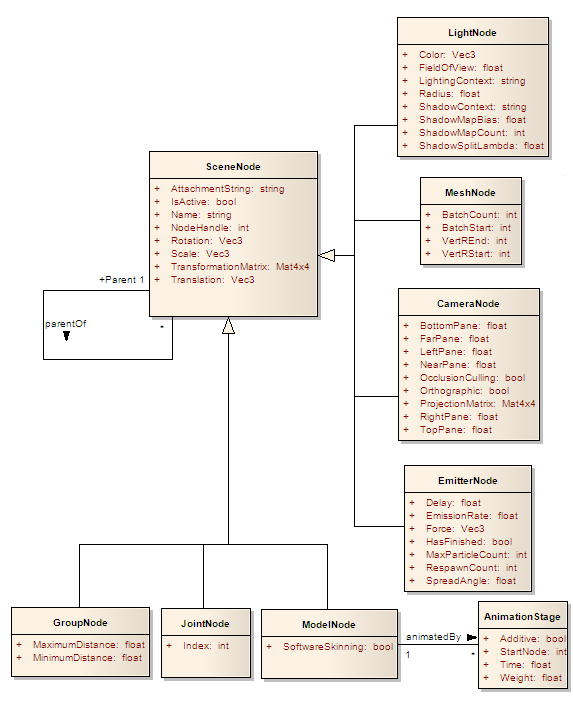
\includegraphics[scale=1.5]{images/Horde3DSceneGraph.png}
%\caption{Aufbau und Vererbungshierarchie des \Horde\ Szenengraphs}\label{fig:h3dscenegraph}
%\end{figure}

Der Szenengraph wird aus folgenden Knotentypen aufgebaut:

\begin{itemize}
	\item \textbf{Group}: Ein \emph{Group Node} hat keine Repr�sentation in der Szene, sondern fasst beliebig viele untergeordnete Knoten zusammen. Damit k�nnen beispielsweise alle untergeordneten Knoten auf einmal in der Szene verschoben, rotiert und ein- oder ausgeblendet werden. \emph{Root Node} ist von diesem Typ.
	\item \textbf{Camera}: In einer Szene k�nnen beliebig viele virtuelle Kameras vorhanden sein, die zum Zeichnen der Szene verwendet werden k�nnen. Insbesondere ist es m�glich, die Kamera einem animierten \emph{Joint Node} unterzuordnen, wobei die Kamera dann dem Bewegungsablauf der Animation folgt.
	\item \textbf{Light}: Ein \emph{Light Node} repr�sentiert eine Lichtquelle in der Szene. Derzeit werden von \Horde\ nur \emph{Spotlights} unterst�tzt. Ein Lichtknoten kann durch verschiedene Parameter -- wie Lichtfarbe, Reichweite und das An- oder Abschalten des Schattenwurfs -- an die Szene angepasst werden.
	\item \textbf{Model}: Ein \emph{Model Node} repr�sentiert ein 3D-Modell, welches aus einer Modellierungssoftware exportiert wurde. Es ist eine Menge von \emph{Mesh Node}s und \emph{Joint Node}s, welche das Aussehen und die Animation des Modells definieren.
	\item \textbf{Mesh}: Ein \emph{Mesh Node} enth�lt verschiedene Polygone, die zum Zeichnen eines 3D-Modells verwendet werden. Alle Polygone werden dabei mit dem gleichen Material gezeichnet.
	\item \textbf{Joint}: Eine Hierarchie von \emph{Joint Node}s repr�sentiert ein animierbares Skelett.
	\item \textbf{Emitter}: Ein \emph{Emitter Node} ist der Ursprungsort von Partikeln und kann verschiedene Eigenschaften der erzeugten Partikel beeinflussen.
	\item \textbf{Overlay}: Ein \emph{Overlay} ist eigentlich kein Teil des Szenengraphs. Es repr�sentiert eine zweidimensionale Grafik, die �ber die dargestellte Szene gezeichnet wird. Damit kann zum Beispiel ein \emph{Heads Up Display} realisiert werden. Auch das Zeichnen von Text wird von \Horde\ durch Verwendung von \emph{Overlay}s umgesetzt.
\end{itemize}

%\begin{figure}[h]
%\centering
%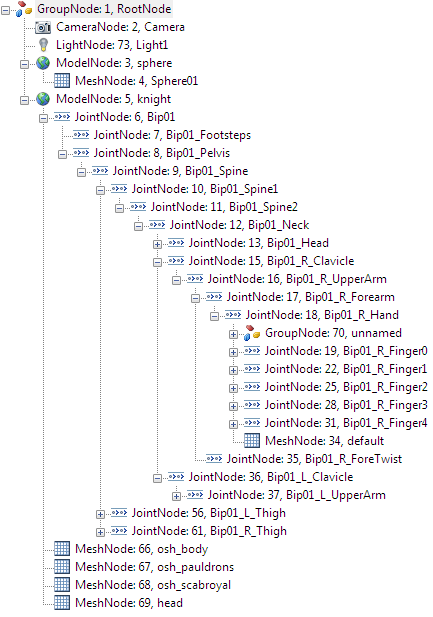
\includegraphics[scale=0.4]{images/KnightSampleSceneGraph.png}
%\caption{Ausschnitt des Szenengraphen des \textit{Horde3D} Knight Samples}\label{fig:knightscenegraph}
%\end{figure}

\subsection{Ressourcen-Verwaltung}
Ressourcen sind Daten, die zum Zeichnen der Szene ben�tigt werden. Dabei k�nnen mehrere \emph{Scene Node}s die gleichen Ressourcen verwenden \cite["`Basic Concepts, Resource Management"']{h3dmanual}. Der Horde3D Ressourcen Manager l�dt Ressourcen bei Bedarf und vergibt eindeutige \emph{Res Handles} zur Identifikation. Ressourcen k�nnen jederzeit neu geladen werden.

Horde3D kennt folgende Arten von Ressourcen:

\begin{itemize}
	\item \textbf{Scene Graph}: Eine \emph{Scene Graph Resource} enth�lt einen Szenengraph, der zum aktuellen Szenengraph als Ast hinzugef�gt werden kann.
	\item \textbf{Geometry}: Eine \emph{Geometry Resource} enth�lt Polygon-Daten f�r \emph{Mesh Nodes}. Neben den eigentlichen Eckpunkt-Koordinaten k�nnen auch weitere Daten -- wie Normalen, Tangenten, Texturkoordinaten, etc. -- enthalten sein.
	\item \textbf{Animation}: Eine \emph{Animation Resource} stellt Animationsdaten f�r \emph{Mesh} und \emph{Joint Nodes} bereit.
	\item \textbf{Pipeline}: Eine \textit{Pipeline Resource} ist ein XML-Dokument, das die erforderlichen Schritte zum Zeichnen der Szene beschreibt. Daf�r k�nnen zun�chst \emph{Render Targets} angelegt und die Engine-Konfiguration angepasst werden. Danach werden die einzelnen Schritte genau beschrieben: Zeichenreihenfolge der Material-Klassen, Lichtberechnungen, Verwenden von \emph{Render Targets} als Quelle und Ziel f�r Zeichenoperation, usw. Die Pipeline ist sehr flexibel und unterst�tzt sowohl \emph{Forward} als auch \emph{Deferred Shading}.
	\item \textbf{Material}: Eine \emph{Material Resource} definiert das Aussehen einer Oberfl�che. Sie legt fest, welche Texturen und welcher Shader zum Zeichnen verwendet werden.
	\item \textbf{Shader}: Eine \emph{Shader Resource} legt einen Kontext f�r die Ausf�hrung der Vertex und Fragment Shader auf der Grafikkarte fest. So kann ein Shader zum Beispiel einen Kontext f�r den \emph{Ambient Pass} und einen f�r den \emph{Deferred Lighting Pass} enthalten. Die Kontexte unterscheiden sich beim Code f�r Vertex und Fragment Shader und bei den Rendering-Optionen wie \emph{Depth Writes}, \emph{Alpha Writes}, etc.
	\item \textbf{Code}: Eine \emph{Code Resource} enth�lt Shader Code, der von mehreren Shadern verwendet werden kann.
	\item \textbf{Texture}: Eine \emph{Texture Resource} ist eine 2D-Textur oder \emph{Cube Map}, die beim Zeichnen von Oberfl�chen verwendet wird.
	\item \textbf{Particle Effect}: Eine \emph{Particle Effect Resource} legt die Gr��e, Farbe, Geschwindigkeit und Lebensdauer von Partikeln fest.
\end{itemize}

%\begin{figure}[h]
%\centering
%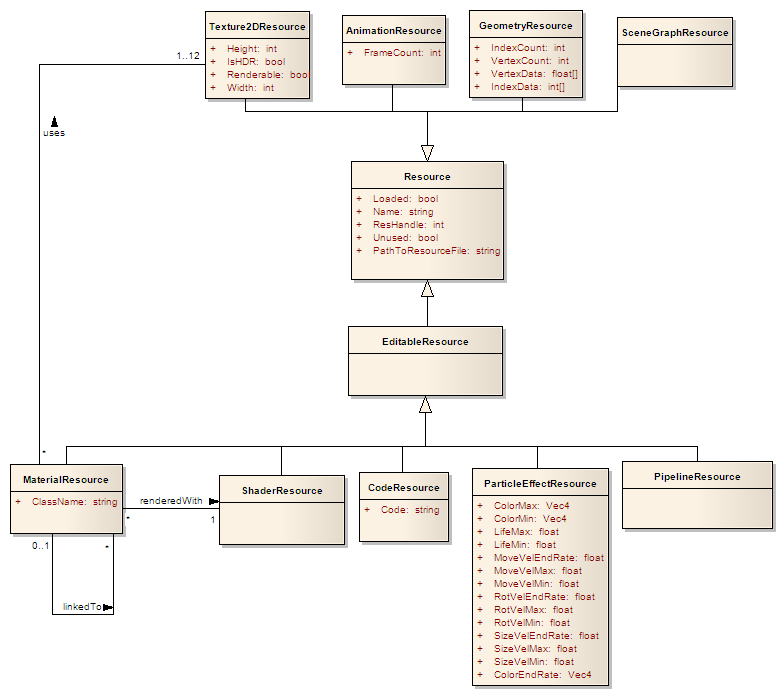
\includegraphics[scale=1.2]{images/Horde3DResources.png}
%\caption{Aufbau und Vererbungshierarchie der \Horde\ Ressourcen}\label{fig:h3dresources}
%\end{figure}

%Abbildung~\ref{fig:h3dresources} beschreibt den Aufbau und Vererbungshierarchie der Ressourcen. Die \textit{EditableResource}-Klasse ist in \textit{Horde3D} nicht vorhanden sondern soll zeigen, welche Arten von Ressourcen vom \DevEnv\ ge�ndert werden k�nnen. Einige Details der Shader und Pipelines sowie der Zusammenhang zwischen Ressourcen und \textit{Scene Nodes} werden in diesem Diagramm aus Gr�nden der �bersichtlichkeit allerdings nicht gezeigt.

\subsection{Eigenschaften der Horde3D-API}
Anwendungen k�nnen \Horde\ durch Einf�gen einer \emph{Header}-Datei und Linken gegen eine \emph{Dynamic Link Library} (DLL) einbinden. Obwohl die Engine in objekt-orientiertem \C++ entwickelt wurde, orientiert sich die �ffentliche Schnittstelle am Design der C-basierten Win32-API. Die Beta 3 von Version 1.0.0 hat gerade einmal 78 �ffentliche Funktionen. Dies erleichtert das Erlernen der API und das Erstellen von \emph{Bindings} f�r verschiedenen Programmiersprachen. Momentan werden C, \C++ und alle .NET-Sprachen offiziell unterst�tzt, weitere \textit{Bindings} werden derzeit von der Community entwickelt\footnote{Momentan entwickelt die Community zum Beispiel \textit{Bindings} f�r die Sprachen Python, D und Lua (\url{http://www.horde3d.org/wiki/index.php5?title=Language_Bindings}). Sogar f�r die funktionale Sprache Haskell gibt es \emph{Bindings} (\url{http://www.horde3d.org/forums/viewtopic.php?f=1&t=550}).}. Gegen�ber einer objekt-orientierten Schnittstelle, wie sie z.B. OGRE bietet, wird f�r manche Aufgaben jedoch mehr Code ben�tigt. Beispielsweise sind drei Funktionsaufrufe n�tig, um die Farbe eines \emph{Light Nodes} zu setzen; die Position, Rotation und Skalierung eines \emph{Nodes} k�nnen nicht einzeln ge�ndert werden und es gibt keine Vektor-Datentypen:

\lstset{language=C++} 
\begin{lstlisting}
// Horde3D::setNodeParamf muss dreimal aufgerufen werden, 
// um die Lichtfarbe auf Rot zu setzen.
Horde3D::setNodeParamf(light, LightNodeParams::Col_R, 1.0f);
Horde3D::setNodeParamf(light, LightNodeParams::Col_G, 0.0f);
Horde3D::setNodeParamf(light, LightNodeParams::Col_B, 0.0f);

// Diese Funktion �ndert die Position, Rotation und Skalierung von 
// 'node'. Daf�r m�ssen immer alle Werte skalar �bergeben werden.
Horde3D::setNodeTransform(node, 0, 20, 50, -30, 0, 0, 1, 1, 1);
\end{lstlisting}

%Wie sich sp�ter jedoch zeigen wird, erleichtert dieser API-Stil die Entwicklung des \DevEnvs.

Die Kern-API wurde schlank gehalten und ist ausreichend, um alle Features der Engine zu verwenden. Es gibt jedoch zus�tzlich die Horde3D \emph{Utility Library}, die verschiedene spezifische Funktionen zur Produktivit�tssteigerung bereitstellt. Mit dieser Bibliothek k�nnen zum Beispiel Ressourcen von der Festplatte geladen, Frame Statistiken angezeigt, der OpenGL-Kontext initialisiert oder Objekte der dargestellten Szene selektiert werden. Der Stil der Horde3DUtils-API entspricht dem der Kern-API \cite["`Utility Library API Reference"']{h3dmanual}.

\Horde\ bietet au�erdem einen Mechanismus an, um die Features der Engine durch Plugins zu erweitern. Diese verwenden nicht die �ffentliche API, sondern haben Zugriff auf die interne Klassenstruktur von \Horde. Um das zu erm�glichen, werden die Plugins zur Kompilierungszeit statisch in die \Horde\ DLL hineinkompiliert. Die �ffentlichen Schnittstellen der Plugins erweitern dann die Kern-API und k�nnen von allen \Horde-Anwendungen verwendet werden, die gegen die erweiterte DLL gelinkt werden \cite["`Basic Concepts"']{h3dmanual}.

\subsection{Fehlerbehandlung und Debug-Informationen}
Da C keine Ausnahmen unterst�tzt, zeigen \Horde-Funktionen Fehler durch spezielle Fehlerwerte auf; so gibt beispielsweise die Funktion \texttt{int getNodeType(NodeHandle)} im Fehlerfall den Wert \texttt{ResourceTypes::Undefined} zur�ck. Zus�tzlich verwaltet \Horde\ intern eine Liste aller aufgetretenen Fehler. Auch Ereignisse und Debug-Informationen werden protokolliert, wie zum Beispiel das Hinzuf�gen eines neuen \emph{Scene Nodes}, das Laden einer Ressource oder Probleme beim Kompilieren des Shader Codes. Die protokollierten Meldungen k�nnen aus der Engine ausgelesen werden, beziehungsweise �ber eine Funktion der \emph{Utility Library} direkt in eine Datei im HTML-Format auf die Festplatte geschrieben werden. Dies sind hilfreiche Informationen beim Entwickeln und Debuggen einer \Horde-Anwendung.

\subsection{Shader und Rendering-Pipeline}
\Horde\ baut auf OpenGL 2.0 auf, das eine hardware-unabh�ngige Schnittstelle f�r hardware-beschleunigte Rasterisierung von 3D-Grafik auf der Grafikkarte (GPU) bietet. Abbildung~\ref{fig:graphicsPipeline} gibt einen �berblick �ber die Pipeline-Architektur moderner GPUs. \texttt{Vertex Data} sind die untransformierten Daten der Eckpunkte der Geometrie der aktuellen Szene. \texttt{Primitive Data} verbindet diese Vertex-Daten zu einer Menge von Punkten, Linien, Dreiecken oder Polygonen. Die \texttt{Vertex Processing}-Stufe verwendet die Szenen- und Projektionsmatrizen zum Transformieren der Eckpunkte und berechnet gegebenenfalls weitere Daten pro Vertex, wie etwa Texturkoordinaten. In der \texttt{Geometry Processing}-Stufe findet die eigentliche Rasterisierung statt. Beim \texttt{Fragment Processing} werden die Farbwerte der Fragmente\footnote{Ein Pixel ist ein Bildpunkt auf dem Bildschirm. Ein Fragment hingegen ist ein Pixel, der eventuell nicht sichtbar ist. Im Allgemeinen werden pro Bild mehr Fragmente berechnet, als Pixel �berhaupt sichtbar sein k�nnen, weil manche Fragmente sp�ter unter gewissen Umst�nden wieder �berschrieben werden.} berechnet und in der \texttt{Fragment Rendering}-Stufe schlie�lich die Tiefen-, Alpha- und \emph{Stencil}-Tests durchgef�hrt. Sind die Tests f�r ein Fragment erfolgreich, so wird es in die Ausgabe-Textur geschrieben oder hineingemischt \cite{dxsdk}.

\begin{figure}[htp]
\centering
%trim=l b r t  	This option will crop the imported image by l from the left, b from the bottom, r from the right, and t  from the top. Where l, b, r and t are lengths. 
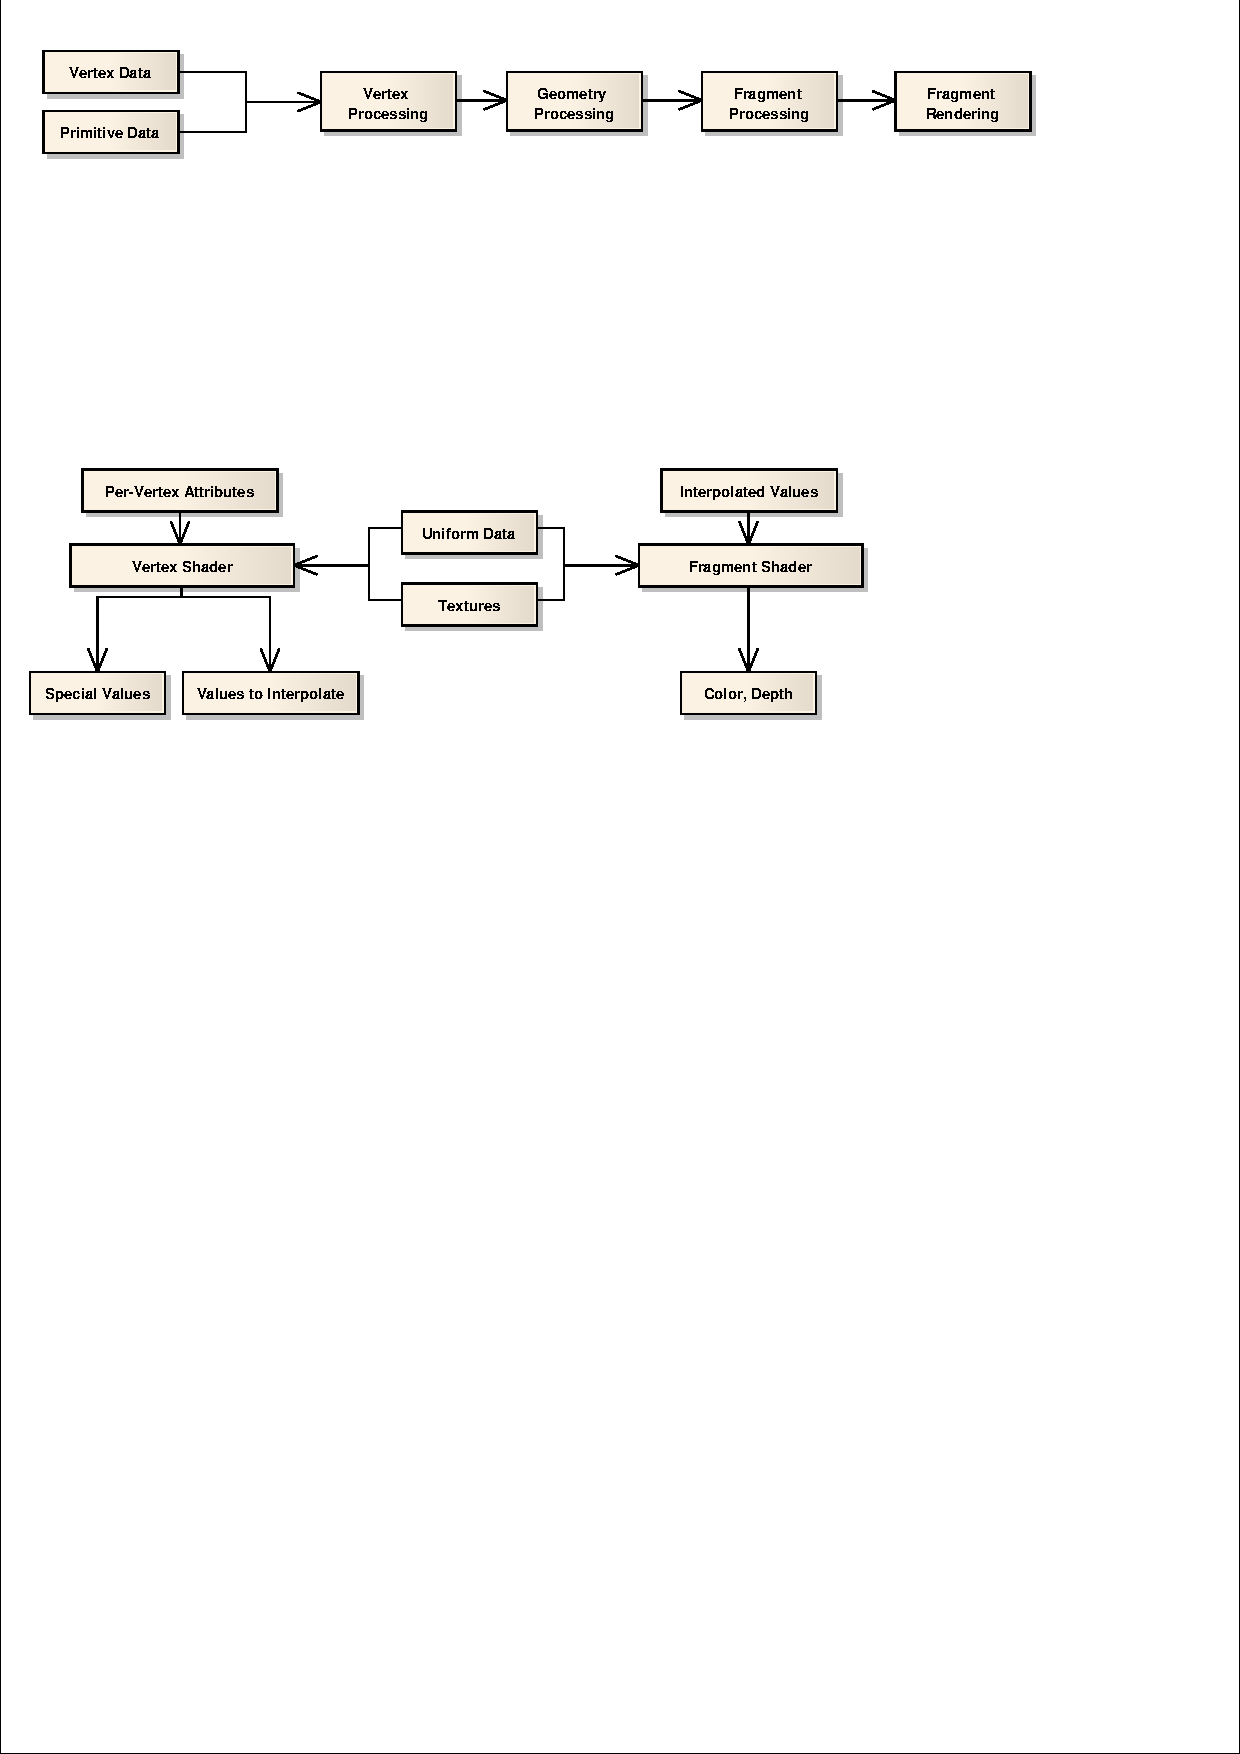
\includegraphics[trim = 5mm 265mm 30mm 5mm, clip, scale=0.7]{images/GraphicsPipeline.pdf}
\caption{Die Grafik-Pipeline von Direct3D 9 und OpenGL 2.0}\label{fig:graphicsPipeline}
\end{figure}

Bei modernen Grafikkarten k�nnen Fragmente nicht nur in den \emph{Backbuffer} geschrieben werden, sondern auch in \emph{Render Targets} (RTs). \emph{Render Targets} k�nnen im weiteren Verlauf wiederum als Eingabe f�r weitere Zeichenoperationen dienen. Dieses Vorgehen ist f�r eine Vielzahl moderner Effekte relevant; beispielsweise gibt es Effekte, die die zuvor berechneten Tiefeninformationen der Szene kennen m�ssen. Es ist auch m�glich, dass eine Zeichenoperation gleichzeitig verschiedene Werte in verschiedene RTs schreibt, also \emph{Multiple Render Target}s (MRTs) verwendet.

Seit DirectX 8 und den \texttt{ARB\_vertex\_program}- und \texttt{ARB\_fragment\_program}-Erweiterungen f�r OpenGL ist es m�glich, die \texttt{Vertex} und \texttt{Fragment Processing}-Stufen der Grafik-Pipeline mit Vertex respektive Fragment Shadern\footnote{Was unter OpenGL Fragment Shader hei�t, wird von Direct3D als Pixel Shader bezeichnet. Da die Fragment/Pixel Shader aber auf Fragmenten und nicht auf Pixeln arbeiten, ist die OpenGL-Terminologie zutreffender.} frei zu programmieren. Allerdings waren diese fr�hen APIs stark eingeschr�nkt; die Syntax der Shadersprache war an Assembler angelehnt und die Anzahl der Instruktionen pro Shader war sehr stark begrenzt. Durch die Weiterentwicklung der Grafik-Hardware konnten die Limitierungen jedoch zunehmend aufgehoben und mit HLSL, Cg und GLSL C-�hnliche Sprachen f�r die Shader-Programmierung entwickelt werden.

Die freie Programmierbarkeit der Vertex und Fragment Shader erm�glicht die Implementierung komplexer, hardware-beschleunigter Effekte. Ohne Shader w�ren die Effekte gar nicht oder nur mit sehr viel Programmieraufwand realisierbar. Der Erfolg der Shader zeigt sich auch dadurch, dass mit DirectX 10 sogar noch eine weitere Shader-Art, Geometry Shader, hinzugekommen ist. Zus�tzlich wurde die \emph{Fixed Function Pipeline}, also die Pipeline ohne frei programmierbare Shader, komplett entfernt. DirectX 11 wird noch drei weitere Shader-Arten hinzuf�gen und HLSL um die Unterst�tzung von objekt-orientierten Konzepten erweitern.

\Horde\ verwendet GLSL als Shadersprache und unterst�tzt derzeit offiziell nur Vertex und Fragment Shader. Wichtig f�r die Verwendung von Shadern ist das Verst�ndnis der Funktionsweise und der Kommunikationsm�glichkeiten zwischen den beiden Shader-Arten. 

Der Shader Code wird f�r jedes Vertex und jedes Fragment einzeln ausgef�hrt, insbesondere kennt ein Shader keine anderen Eckpunkte oder Fragmente. Nur durch diese Einschr�nkung kann der hohe Grad der Parallelisierbarkeit der Shader gew�hrleistet werden -- moderne Grafikkarten berechnen hunderte Shader gleichzeitig. 

\begin{figure}[htp]
\centering
%trim=l b r t  	This option will crop the imported image by l from the left, b from the bottom, r from the right, and t  from the top. Where l, b, r and t are lengths. 
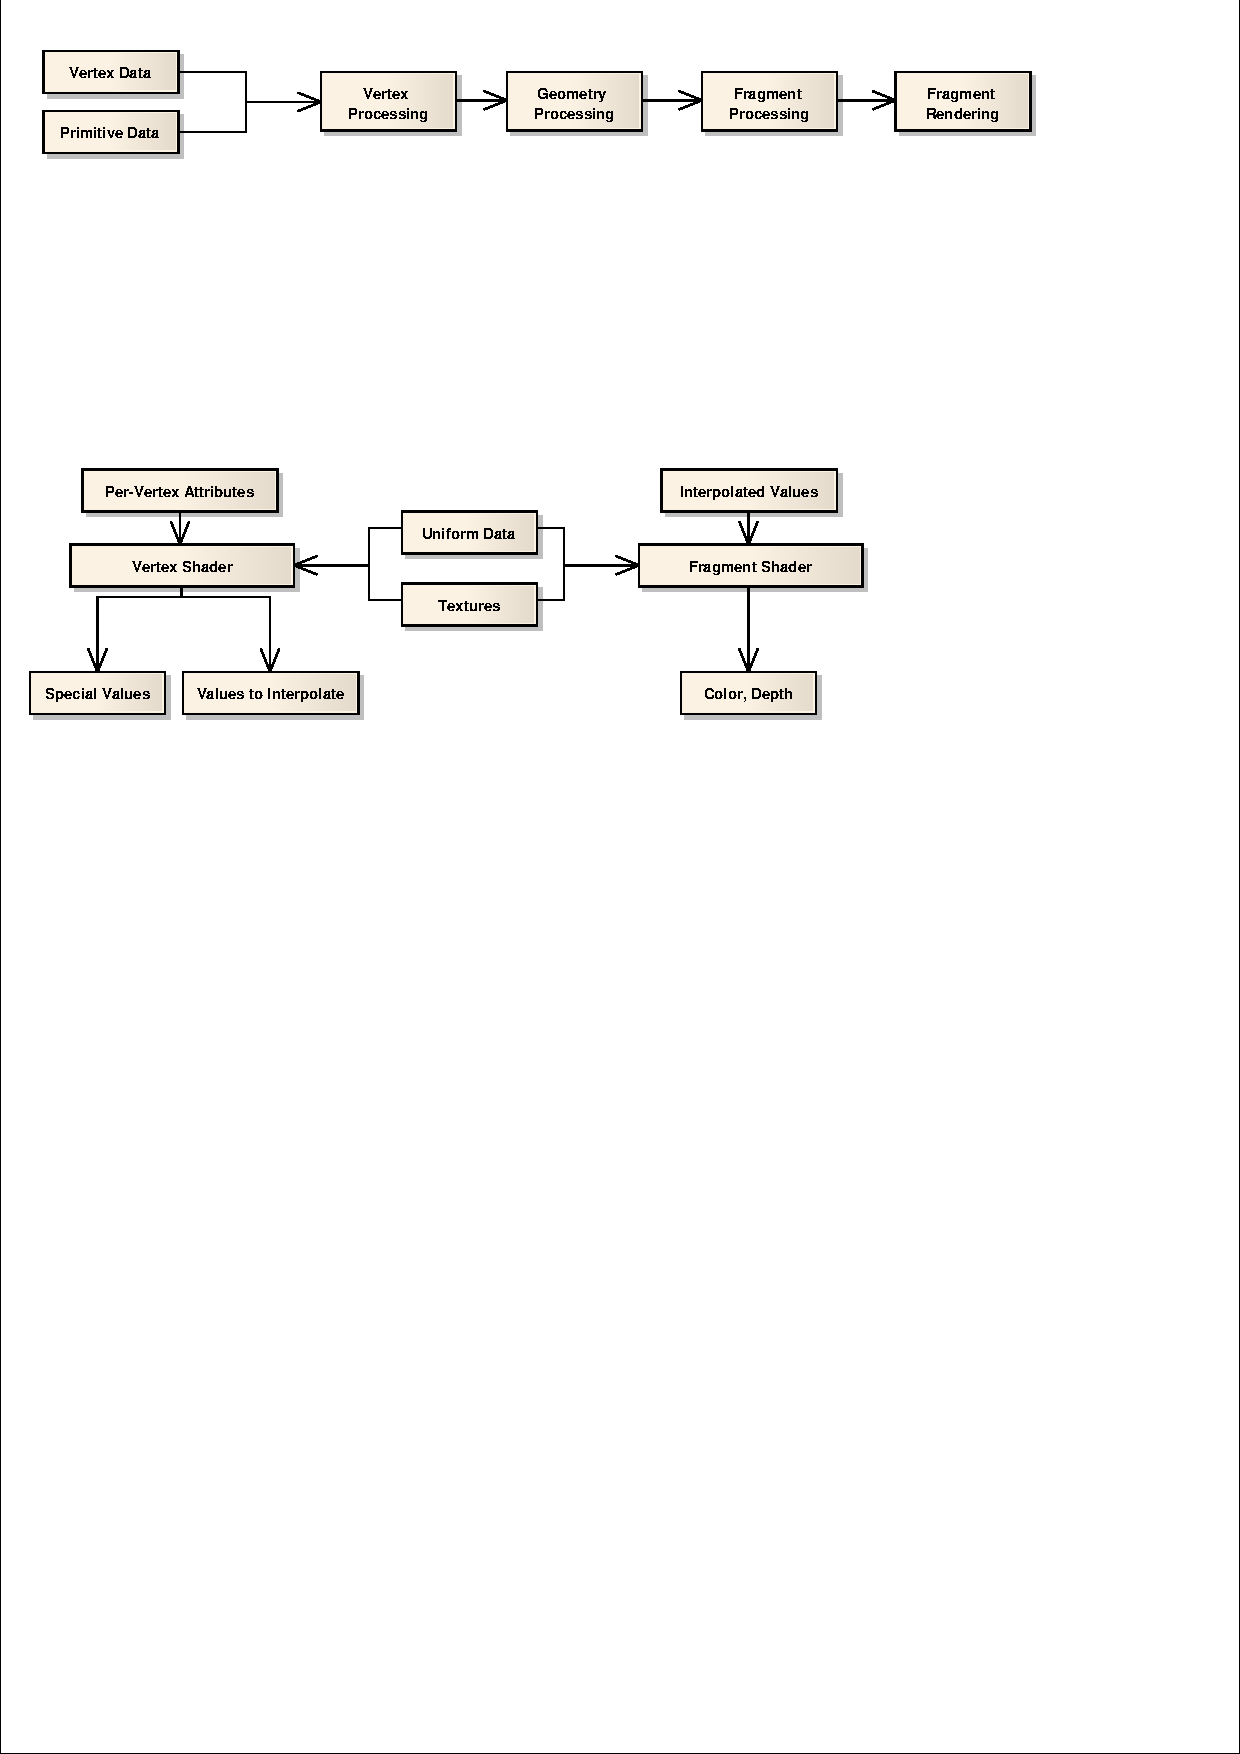
\includegraphics[trim = 5mm 170mm 45mm 75mm, clip, scale=0.7]{images/GraphicsPipeline.pdf}
\caption{Datenfluss zwischen Vertex und Fragment Shadern in OpenGL 2.0}\label{fig:shaderData}
\end{figure}

Abbildung~\ref{fig:shaderData} zeigt den Datenfluss zwischen den Shadern. Der Vertex Shader erh�lt Attribute f�r jedes Vertex, beispielsweise die Position und die Textur-Koordinaten. �ber \emph{Uniform}s k�nnen Vertex-unabh�ngige Daten, wie etwa die Transformations- und Projektionsmatrizen, Position der Lichtquelle, etc., abgerufen werden. Manche \emph{Uniform}s werden von OpenGL auch als \emph{built-in} Variablen zur Verf�gung gestellt\footnote{\emph{Built-in} Variablen wie beispielsweise Nebel- oder Lichtquellen-Einstellungen sind aus Effizienzgr�nden seit OpenGL 3.1 kein Teil des Standards mehr \cite{openglspec}.}. Auch Texturen k�nnen als Eingabe verwendet werden. Die Ausgabe erfolgt an spezielle Ausgabevariablen oder an Variablen, die �ber alle Eckpunkte eines Primitivs interpoliert und an den Fragment Shader weitergereicht werden. Der Fragment Shader kann mit diesen interpolierten Werten weiterrechnen und hat ebenfalls Zugriff auf die \emph{Uniforms}. Die Ausgabe des Fragment Shaders ist ein Farbwert und implizit auch ein Tiefenwert. Bei der Verwendung von MRTs werden mehrere Farbwerte ausgegeben \cite[S. 52]{astle}.

\Horde\ verwendet zwar GLSL, f�hrt aber ein XML-�hnliches Format ein, um die Ausdrucksst�rke der Shader zu erweitern. Die Erweiterung ist an die \emph{HLSL Effects} von Direct3D angelehnt. Dieses Framework erm�glicht es, f�r einen Effekt verschiedene Stufen zu definieren -- von \Horde\ als Kontext bezeichnet --, die jeweils unterschiedlichen Shader Code ausf�hren. Es k�nnen auch \emph{Uniforms} global definiert und Einstellungen f�r verwendete Texturen, wie zum Beispiel der anzuwendende Texturfilter, festgelegt werden. Jeder Kontext kann au�erdem die Vergleichsfunktion f�r den Tiefen- und Alphatest ausw�hlen und eine Funktion f�r das \emph{Blending} spezifizieren.

Das Pipeline-Konzept von \Horde\ geht jedoch �ber die \emph{HLSL Effects} hinaus. Pipelines erm�glichen die Definition verschiedener \emph{Render Targets} und die Festlegung deren Verwendung in den einzelnen Zeichenschritten als Ein- oder Ausgabe f�r die Shader. Es kann genau spezifiziert werden, welche Material-Klassen mit welchen Shader-Kontexten gezeichnet werden, wann \emph{Overlays} �ber die Szene gelegt werden und welche Art der Lichtberechnung -- \emph{Forward} oder \emph{Deferred Shading} -- verwendet wird. 
\section{Anforderungen an das System}
\begin{figure}[ht]
\centering
%trim=l b r t  	This option will crop the imported image by l from the left, b from the bottom, r from the right, and t  from the top. Where l, b, r and t are lengths. 
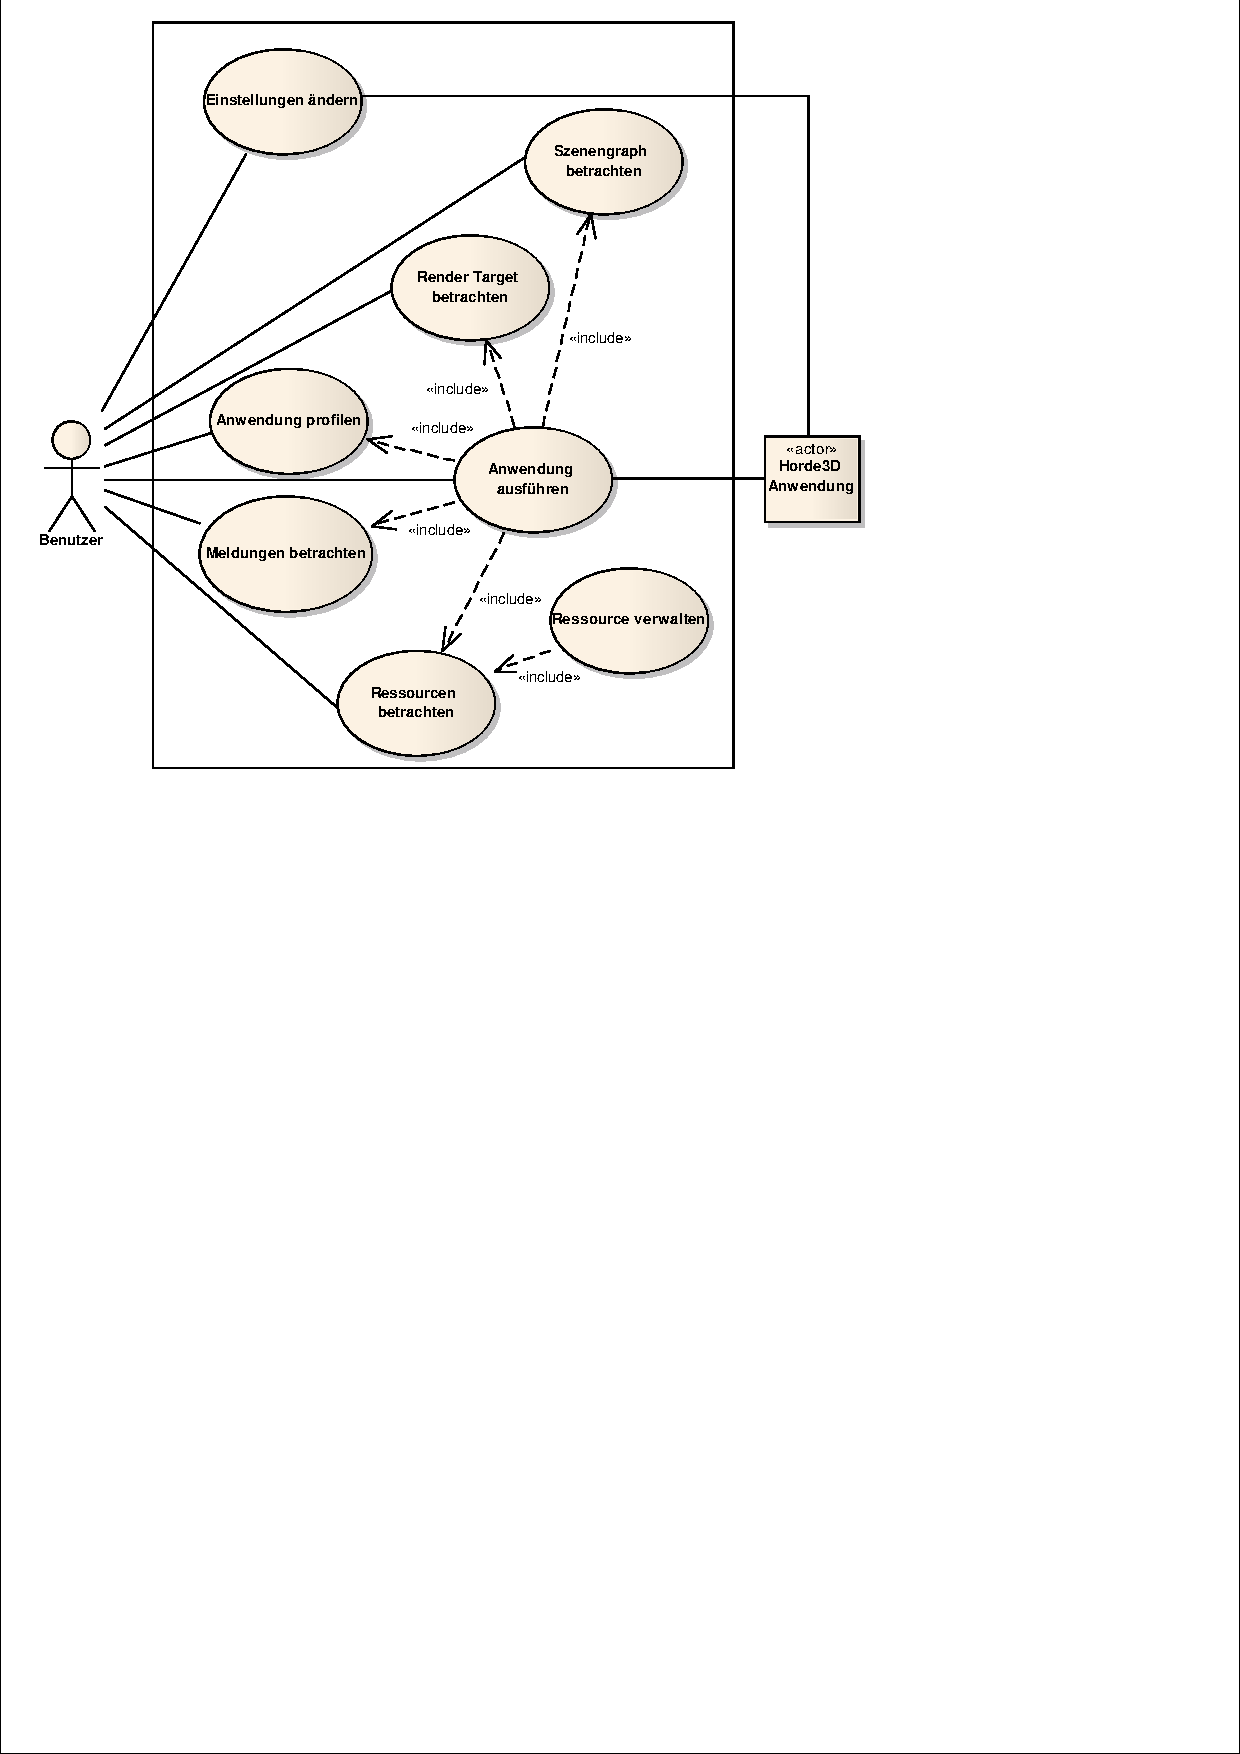
\includegraphics[trim = 1mm 160mm 60mm 1mm, clip, scale=0.7]{images/UseCase_Model.pdf}
\caption{Das \emph{Use Case} Modell des \DevEnvs}\label{fig:ucModel}
\end{figure}
Nach der Betrachtung der Funktionsweise von \Horde\ mussten die Anforderungen an das \DevEnv\ konkretisiert werden. Es kamen viele M�glichkeiten in Betracht, die Entwickler eines Spiels beim Erstellen, Optimieren und Feinabstimmen der Spieleeffekte zu unterst�tzen. Im Rahmen dieser Bachelorarbeit wurden deshalb ausschlie�lich diejenigen Anforderungen betrachtet, die speziell bei der Entwicklung von \SheepMeUp\ von Nutzen gewesen w�ren. Weitere denkbare Anforderungen und Erweiterungen des Systems werden in Kapitel~\ref{Ausblick} vorgestellt.

Abbildung~\ref{fig:ucModel} zeigt das \emph{Use Case} Modell des Systems. Die Anwendungsf�lle werden in den folgenden Abschnitten genauer beschrieben. Aktivit�tsdiagramme f�r die \emph{Use Cases} sind im Anhang abgebildet.

\subsection{Unabh�ngigkeit und Eigenst�ndigkeit}
Eine �bergeordnete Anforderung an das System war die Unabh�ngigkeit von der konkreten \Horde-Anwendung und von der Implementierung von \Horde. Um das \DevEnv\ beim Entwickeln einer Anwendung verwenden zu k�nnen, sollen keine �nderungen an der Anwendung n�tig sein; es sollen keine speziellen Funktionen aufgerufen oder gegen zus�tzliche Programmbibliotheken gelinkt werden m�ssen. 

Das System soll aber auch unabh�ngig von der Implementierung von \Horde\ sein. Dies verhindert das �berladen der Kern-API der Engine mit Tool-spezifischen Funktionen und erleichtert die Weiterentwicklung in getrennten Entwicklergruppen. 

Einzige Voraussetzung an \Horde-Anwendungen ist, dass eine unmodifizierte Horde3D DLL verwendet wird\footnote{Die derzeitige Implementierung unterst�tzt ohne erneutes Kompilieren keine modifzierten \Horde\ DLLs oder \Horde-Extensions.}.

\subsection{Absicherung vor unerw�nschtem Reverse-Engineering}
Mit dem \DevEnv\ k�nnen Einblicke in den Aufbau und in die Funktionsweise der Effekte von \Horde-Anwendung gewonnen werden. Dies k�nnte m�g\-lich\-er\-weise von manchen Anwendungsentwicklern unerw�nscht sein. Das System soll seine Dienste verweigern, wenn die Anwendung die Verwendung des \DevEnvs\ nicht explizit erlaubt. Um die Verwendung nur explizit zuzulassen, ist jedoch eine Modifizierung der Anwendung notwendig. Die damit einhergehende Verletzung des Ziels der Unabh�ngigkeit wird aber bewusst in Kauf genommen. So soll es f�r die Entwickler von \Horde-Anwendungen m�glich sein, das \DevEnv\ nur mit \emph{Debug Builds} ihrer Anwendung zu verwenden, wohingegen das Tool bei \emph{Release Builds} nicht verwendet werden kann.

Diese Anforderung wurde erst in einer sp�teren Iteration aufgenommen. Urspr�nglich regte Nicolas Schulz, der Entwickler von \Horde, die Entwicklung des Schutzmechanismus an.

\subsection{Konfigurieren und Ausf�hren der Horde3D-Anwendung}
Das System soll als eigenst�ndig ausf�hrbares Programm entwickelt werden, aus dem heraus die \Horde-Anwendung gestartet werden kann. Dadurch wird es erleichtert, die Anforderung der Unabh�ngigkeit zu erf�llen. Eine Alternative w�re, w�hrend der Ausf�hrung der Anwendung beim Dr�cken einer bestimmten Taste das \DevEnv\ zu laden und anzuzeigen. Dies h�tte jedoch �nderungen an der Anwendung oder an \Horde\ notwendig gemacht. Ein weiterer Vorteil der gew�hlten L�sung ist die M�glichkeit, das Tool sp�ter auch "`offline"' -- also ohne laufende \Horde-Anwendung -- verwenden zu k�nnen (siehe auch Kapitel~\ref{Ausblick}).

F�r den Start der \Horde-Anwendung sollen verschiedene Parameter eingestellt und gespeichert werden k�nnen: der Pfad zur \emph{Executable} der Anwendung, das Arbeitsverzeichnis, Kommandozeilenparameter sowie verschiedene implementierungsspezifische Details. Das \DevEnv\ soll eine Eingabemaske f�r diese Parameter bereitstellen und die Pfade auf Korrektheit �berpr�fen. Abbildung~\ref{fig:ucEinstellungenAendern} zeigt das Aktivit�tsdiagramm f�r die Konfiguration der Anwendungsparameter.

Abbildung~\ref{fig:ucAnwendungAusfuehren} erl�utert die Verwendung des \DevEnvs. Das System soll auf Wunsch des Benutzers die Anwendung starten. Der Benutzer soll grunds�tzlich jederzeit die M�glichkeit haben, die Anwendung wieder zu beenden. W�hrend das Programm l�uft, soll das System sofort alle von \Horde\ generierten Fehler-, Debug- und Informationsmeldungen in einer �bersicht anzeigen. Damit kann der Benutzer Probleme seiner Anwendung identifizieren, ohne die von den Horde3DUtils generierte HTML-Datei durchzusehen.

Hat die Anwendung einen Zustand erreicht, in dem der Benutzer die Anwendung anhalten m�chte, teilt er dies dem System mit. Das System soll die Anwendung anhalten und es dem Benutzer erm�glichen, die aktuelle Szene zu betrachten und Ressourcen zu �ndern, w�hrend sich die Szene selbst nicht �ndert. Dies kann im Allgemeinen, also ohne ein spezielles Anhalten der Anwendung, nicht garantiert werden: Ein Explosionseffekt in einem Spiel wird beispielsweise nur wenige Sekunden andauern. M�chte man den Effekt �ndern, so kann das Anhalten der Explosionsanimation beim Finetuning der Details der Explosion hilfreich sein.

W�hrend die Szene eingefroren ist, soll der Benutzer den Zustand der Anwendung analysieren k�nnen:

\begin{itemize}
	\item Das System soll alle bekannten Ressourcen auflisten. Falls eine Ressource editierbar ist, soll auf Wunsch die XML-Datei der Ressource geladen werden k�nnen. Der Benutzer soll die XML-Datei frei �ndern und die �nderungen speichern k�nnen. Anschlie�end soll das System die Szene mit der ge�nderten Ressource automatisch neu zeichnen.

	\item W�hrend der Ausf�hrung der Anwendung werden von \Horde\ Fehler- und Debug-Meldungen erzeugt. Das System soll diese bereits w�hrend der Ausf�hrung anzeigen und eine Filterung nach Wichtigkeit unterst�tzen.
	
	\item %Viele Shader-Effekte ben�tigen eine Kopie der aktuellen Szene. Daf�r werden Render Targets verwendet: Die Szene wird zun�chst in ein Render Target gezeichnet, aus welchem anschlie�end ein Shader die Szenendaten auslesen kann. Die Rendering Pipeline von \Horde\ unterst�tzt dieses Prinzip. 
	Mit dem Tool soll es m�glich sein, den Inhalt von aktiven \emph{Render Targets} zu betrachten. Da sich deren Daten, w�hrend die Anwendung nicht eingefroren ist, in jedem Frame �ndern k�nnen, soll das System automatisch in kurzen Zeitintervallen den dargestellten Inhalt aktualisieren.
	
		\item Das \DevEnv\ soll dem Benutzer eine einfache Profiling-Funktion anbieten. Das System soll die Aufrufe aller \Horde-Funktionen aufzeichnen und dem Benutzer anzeigen. Es soll dann eine Auswertung der gewonnenen Daten m�glich sein.

	\item Der Benutzer soll einen �berblick �ber den aktuellen Zustand des Szenengraphs erhalten k�nnen. Dazu soll der komplette Szenengraph als Baum dargestellt werden. Zu jedem \emph{Scene Node} sollen auf Wunsch weitere Details, wie etwa Typ, Name, Transformationswerte, etc., angezeigt werden. 
	
\end{itemize}

Anschlie�end kann der Benutzer entweder die Anwendung beenden oder mit der Ausf�hrung fortfahren. Anders als in Abbildung~\ref{fig:ucAnwendungAusfuehren} dargestellt, soll das System aber auch w�hrend der Weiterausf�hrung das �ndern von Ressourcen und Anzeigen des Inhalts von \emph{Render Targets} erlauben.

\subsection{Bearbeiten von Ressourcen und sofortiges Anzeigen der �nderungen}
Das System soll das Neuladen von ge�nderten Ressourcen ohne explizite Unterst�tzung der Anwendung erm�glichen. Das ist der wichtigste \emph{Use Case} des \DevEnvs: Jeder beliebige Shader- oder Partikel-basierte Spezialeffekt, jedes Material und jede Pipeline soll mit dem Tool zur Laufzeit der Anwendung, aber v�llig unabh�ngig von dieser, ge�ndert werden k�nnen. Die Anwendung soll beim n�chsten Zeichnen der Szene sofort die aktualisierten Ressourcen verwenden. Abbildungen \ref{fig:ucRessourcenBetrachten} und \ref{fig:ucRessourceVerwalten} zeigen den Ablauf dieses Anwendungsfalls. Zun�chst sollen alle Ressourcen in einer �bersicht angezeigt werden. Das System soll eine Filterm�glichkeit nach Ressourcen-Typ und -Name anbieten. Falls der Benutzer eine editierbare Ressource ausw�hlt, soll das System die zugrundeliegende XML-Datei der Ressource in einem Texteditor anzeigen. �nderungen an der XML-Datei sollen gespeichert und sofort an die \Horde-Anwendung �bermittelt werden k�nnen.

Beim Entwickeln der Kraftfeld- und Schockwellen-Effekte f�r \SheepMeUp\ war es wichtig, verschiedene Parameter der Effekte fein zu justieren und an das \emph{Look and Feel} des Spiels anzupassen. Das Ausblenden des Effekts, die Farbgebung, die Intensit�t und die Abspieldauer mussten von Hand eingestellt werden. Da weder \Horde\ noch \SheepMeUp\ ein automatisches Neuladen der Ressourcen unterst�tzen, war nur folgendes Vorgehen m�glich:

\begin{enumerate}
	\item Die XML-Datei des Effekts �ndern.
	\item Eventuell muss die Anwendung neu kompiliert und gelinkt werden\footnote{Bei der Entwicklung von \SheepMeUp\ war eine Neukompilierung erforderlich, wenn der Effekt von Werten aus der Anwendung abhing, die ebenfalls angepasst werden mussten. Dieses Problem kann das \DevEnv\ nicht l�sen. W�re \SheepMeUp\ nicht in \C++, sondern in \Csharp\ entwickelt worden, h�tte dieses Problem durch die \emph{Edit And Run}-Funktionalit�t von Visual Studio vermieden werden k�nnen.}.
	\item Das Spiel starten.
	\item Bis zur entsprechenden Stelle im Spiel spielen.
	\item Das Aussehen des Effekts beurteilen.
	\item Bei Nichtgefallen zur�ck zu Schritt 1.
\end{enumerate}

Dieser Prozess war zeitintensiv und unproduktiv. Das \DevEnv\ soll ein kontinuierliches Testen und Anpassen der Effekte erm�glichen und somit die Optimierung der Effekte leichter und schneller gestalten. Dies f�hrt zu einer entsprechenden Verbesserung der �sthetik des Spiels, und somit auch des Spiels insgesamt \cite[nach S. 89]{schell}. Das verbesserte Vorgehen l�sst sich wie folgt zusammenfassen:

\begin{enumerate}
	\item Das Spiel starten. 
	\item Bis zur entsprechenden Stelle im Spiel spielen.
	\item Das Aussehen des Effekts beurteilen.
	\item Die XML-Datei des Effekts �ndern, gegebenenfalls sogar unterst�tzt durch einen Designer.
	\item Bei Nichtgefallen zur�ck zu Schritt 3.
\end{enumerate}

W�hrend der Entwicklung des Systems zeigte sich au�erdem, dass das Shader-Format von \Horde\ bei komplexen Shadern un�bersichtlich werden kann. Aus diesem Grund wurde die Entwicklung eines visuellen Designers f�r \Horde-Shader in die Anforderungen aufgenommen. Im Rahmen dieser Bachelorarbeit soll die n�tige Infrastruktur f�r den Shader-Designer implementiert sowie die automatische Synchronisation des Designers und der XML-Datei umgesetzt werden. Der Designer soll das �ndern von bereits vorhandenen Shadern unterst�tzen; neue Shader sollen damit nicht angelegt werden k�nnen. In Kapitel~\ref{Ausblick} wird kurz auf die Limitierungen der derzeitigen Implementierung des Designers eingegangen.

\subsection{Anzeigen von Fehlern und Debug-Informationen}
\Horde\ generiert laufend Fehler- und Debug-Meldungen. Diese Meldungen sind die einzige M�glichkeit, mehr �ber aufgetretene Probleme beziehungsweise den derzeitigen internen Zustand der Engine zu erfahren. So traten bei der Entwicklung von \SheepMeUp\ mehrere Probleme auf, die nur mit Hilfe von \Horde-Fehlermeldungen gel�st werden konnten. Beispielsweise kam es in unregelm��igen Zeitabst�nden vor, dass scheinbar zuf�llig ausgew�hlte Schafe aus der Szene entfernt wurden. Im Anwendungscode gab es keine Hinweise, die dieses Problem erkl�ren konnten, da Schafe nur an einer genau definierten Stelle gel�scht wurden. Der entsprechende Code wurde beim Auftreten des Bugs aber nicht ausgef�hrt. Erst ein Blick in die von den Horde3DUtils generierte HTML-Datei f�hrte zur L�sung des Problems. Die Datei enthielt mehrere Warnungen �ber Versuche, \emph{Scene Nodes} �ber ung�ltige \emph{Node Handles} aus dem Szenengraph zu l�schen. Es stellte sich heraus, dass die Schafe sowohl vom Anwendungscode gel�scht wurden als auch von der verwendeten Game Engine der Universit�t Augsburg. Da \Horde\ nach dem L�schen eines Knoten dessen \emph{Node Handle} neu vergibt, wurde manchmal beim zweiten L�schen ein neu erzeugter Knoten im Szenengraph gel�scht. Mit diesem Wissen war das Problem leicht zu beheben und die HTML-Datei war anschlie�end frei von Fehlermeldungen.

Die Wichtigkeit der \Horde-Meldungen beim Entwickeln von Anwendungen ist nicht zu untersch�tzen. Problematisch ist, dass die Meldungen standardm��ig gar nicht angezeigt werden und von den Horde3DUtils nur in eine HTML-Datei geschrieben werden. Dort aber �bersieht man wichtige Informationen leicht. Im Zusammenhang mit dem Neuladen von aktualisierten Ressourcen sind die Meldungen aber auch noch aus einem weiteren Grund sehr wichtig. Sie zeigen n�mlich Probleme beim Neuladen der Ressourcen an, beispielsweise Syntaxfehler im GLSL-Code oder falsche Pfade zu referenzierten Ressourcen. 

Das System soll zum einen alle generierten Meldungen anzeigen und zum anderen auch das Filtern der Meldungen nach Wichtigkeit -- also Fehler, Warnung, Debug-Information -- unterst�tzen. Abbildung~\ref{fig:ucMeldungenBetrachten} zeigt das Aktivit�tsdiagramm f�r diesen \emph{Use Case}.

\subsection{Anzeigen von Render Targets}
F�r die Kraftfeld- und Schockwellen-Effekte verwendet \SheepMeUp\ mehrere \emph{Render Targets}, die die aktuellen Szenen-Daten, den Abstand eines Pixels zur Kamera und Ergebnisse verschiedener Zwischenberechnungen enthalten. Beim Programmieren der Shader w�re es hilfreich gewesen, direkt den Inhalt der RTs betrachten zu k�nnen. Als Workaround musste ein spezieller Schritt in die Pipeline-Konfiguration von \SheepMeUp\ eingef�hrt werden, der den Inhalt eines \emph{Render Targets} in den \emph{Backbuffer} kopiert und anzeigt. Das Spiel musste dann neu ge\-star\-tet und bis zur entsprechenden Stelle gespielt werden, um den Inhalt des RTs betrachten zu k�nnen. 

\emph{Render Targets} werden generell f�r die Grafikentwicklung immer wichtiger. \emph{Post Processing} Shader ben�tigen die gezeichnete Szene als Eingabe und das immer mehr in Mode kommende \emph{Deferred Shading} ben�tigt MRTs, um die Position jedes Pixels in der 3D-Welt, die Normale des Pixels und Materialeigenschaften zu speichern \cite[S. 255ff]{astle}. Daher soll das \DevEnv\ das Betrachten des RT-Inhalts vereinfachen. Wie Abbildung~\ref{fig:ucRenderTargetBetrachten} zeigt, soll das System dem Benutzer alle bekannten \emph{Render Targets} der eingefrorenen Szene zur Auswahl anbieten. Nachdem der Benutzer eines ausgew�hlt hat, soll das Tool den Inhalt des RTs darstellen. Da sich dieser im Allgemeinen in jedem Frame �ndert, soll das System immer die aktuellen Daten anzeigen. Dies soll auch w�hrend der Ausf�hrung der Anwendung m�glich sein. Bei der Implementierung dieses Features zeigte sich jedoch, dass ein Auslesen der RT-Daten in Echtzeit zu unperformant ist. Stattdessen soll ein Intervall eingestellt werden k�nnen, innerhalb dessen die angezeigten Daten aktualisiert werden.

\subsection{Profiling von Horde3D-Funktionen}
Grafikberechnungen sind sehr leistungshungrig, daher kann eine Optimierung des Codes lohnend sein -- eventuell gest�tzt durch Profiling-Tools wie Intels VTune\footnote{\url{http://software.intel.com/en-us/intel-vtune}}. Es ist keine Anforderung an das \DevEnv, etablierte Profiling-Tools zu ersetzen. Es soll aber m�glich sein, einen generellen �berblick �ber die Aufrufkosten von \Horde-Funktionen zu erhalten und entsprechende Auswertungen vorzunehmen. Das System soll eine Szene profilen k�nnen, indem es f�r einen Frame die Aufrufdaten der \Horde-Funktionen -- den Zeitpunkt des Aufrufs, die Ausf�hrungsdauer, sowie die Aufrufsreihenfolge und damit die Aufrufsh�ufigkeit -- protokolliert und dem Benutzer anzeigt. Der Benutzer soll die gewonnen Daten nach folgenden Kriterien analysieren k�nnen: Durchschnittliche Ausf�hrungsdauer einer Funktion, absolute Ausf�hrungsdauer einer Funktion und Anzahl der Aufrufe einer Funktion. Es soll au�erdem eine Aufruf-Historie dargestellt werden, die den zeitlichen Ablauf der Funktionsaufrufe repr�sentiert. Abbildung~\ref{fig:ucAnwendungProfilen} zeigt diesen Anwendungsfall als Aktivit�tsdiagramm.

\subsection{Anzeigen des Szenengraphs}
Im Rahmen der Bachelorarbeit soll eine Visualisierung des Zustands des Szenengraphs einer eingefrorenen Szene implementiert werden. Die Visualisierung soll dabei die Baumstruktur des Szenengraphs widerspiegeln. Wie Abbildung~\ref{fig:ucSzenengraphBetrachten} illustriert, sollen zu jedem \emph{Scene Node} auf Wunsch des Benutzers weitere Details angezeigt werden, wie beispielsweise der Typ des Knotens, sein Name oder seine Transformationswerte. F�r das Auslesen und Anzeigen der Daten soll die ben�tigte Infrastruktur entworfen und implementiert werden. In Kapitel~\ref{Ausblick} werden Ideen und M�glichkeiten f�r zuk�nftige Versionen des Tools vorgestellt, um diese Daten f�r interessante und hilfreiche Features zu verwenden.
\section{Konzeptmodell}

Abbildung~\ref{fig:domainModel} zeigt das Konzeptmodell des \DevEnvs. Die meisten Konzepte, ihre Abh�ngigkeiten und Spezialisierungshierarchien wurden von der Struktur und vom Aufbau von \Horde\ vorgegeben. Das Modell musste nur um die Konzepte \texttt{Horde3DApplication}, \texttt{FunctionCall} und \texttt{EditableResource} erweitert werden. Ersteres repr�sentiert die Anwendung, die vom Tool gestartet wird. \texttt{FunctionCall} wurden gegen�ber den System-Anforderungen noch um die Attribute \texttt{ReturnValue} und \texttt{Parameters} erweitert. In diesen beiden Attributen werden die Werte, die an die Funktion �bergeben beziehungsweise von ihr zur�ckgegeben werden, aufgezeichnet. Diese Daten wurden erst in einer sp�teren Iteration ins Konzeptmodell aufgenommen. Damit wird eine der in Kapitel~\ref{Ausblick} beschriebenen Erweiterungen bereits vorbereitet.

Im Konzeptmodell wurden alle Typen von \emph{Scene Nodes} als Spezialisierungen des abstrakten Konzepts \texttt{SceneNode} dargestellt. Bei den Ressourcen wurde zus�tzlich noch das Konzept der editierbaren Ressource hinzugef�gt, da das \DevEnv\ nur gewisse Ressourcentypen -- Materials, Pipelines, Shaders, Particle Effects und Code Ressourcen -- ver�ndern kann. Alle editierbaren Ressourcen sind durch das abstrakte Konzept \texttt{EditableResource} generalisiert, w�hrend alle anderen Ressourcen und \texttt{EditableResource} selbst Spezialisierungen des allgemeineren abstrakten Konzepts \texttt{Resource} sind.

Es wurden au�erdem die Beziehungen der einzelnen Ressourcen untereinander untersucht. Die Pipeline Konfiguration wurde auf einzelne Konzepte aufgeteilt, um m�glichst flexibel auf �nderungen und Erweiterungen der Pipeline in neuen \Horde-Versionen reagieren zu k�nnen. Au�erdem wurden die Assoziationen zwischen den \emph{Scene Nodes} und ihren ben�tigten Ressourcen eingezeichnet. Damit wird es sp�ter m�glich sein, f�r einen \emph{Scene Node} die verwendeten Ressourcen zu betrachten beziehungsweise f�r eine Ressource herauszufinden, von welchen Teilen des Szenengraphs sie verwendet wird. Diese detaillierte Analyse der Assoziationen zwischen den Konzepten war zwar nicht aufgrund der \emph{Use Cases} erforderlich, verbesserte aber das Verst�ndnis des Problembereichs und wird f�r einige der vorgeschlagenen Erweiterungen in Kapitel~\ref{Ausblick} ben�tigt.

Die \Horde-Konzepte, ihre Attribute und ihre Abh�ngigkeiten untereinander wurden aus der API-Beschreibung der \Horde-Dokumentation \cite["`Engine API Reference"']{h3dmanual} ermittelt. Da w�hrend der Entwicklung der Anwendung eine neue \Horde-Version erschien, mussten in einer sp�teren Iteration einige wenige Details der Konzepte ver�ndert werden. Hierbei machte sich allerdings die starke Modularisierung des Konzeptmodells positiv bemerkbar.
\section{Verwandte Softwaretools}\label{abgrenzung}
Neben dem \DevEnv\ gibt es eine Reihe weiterer Tools mit dem Ziel, die Entwicklung von 3D-Anwendungen zu vereinfachen und zu beschleunigen. Dabei unterscheiden sich die Tools nicht nur in ihrer Umsetzung, sondern vor allem auch darin, welches Problem sie zu l�sen versuchen. 

Nachdem die erste Iteration der Analyse abgeschlossen war, wurden die gefundenen Anforderungen mit bereits vorhandenen Tools verglichen. Teilweise dienten Ideen anderer Tools als Grundlage f�r Erweiterungen und Erg�nzungen der Anforderungen w�hrend der zweiten Iteration der Analyse-Phase. Es konnten aber auch Ideen f�r die Design- und Implementierungs-Phasen gewonnen werden.

Die folgenden Tools wurden eingehender betrachtet. Es wird kurz auf den Verwendungszweck, die Unterschiede zum \DevEnv\ und auf die f�r die weitere Entwicklung hilfreichen Ideen eingegangen.

\subsection{Horde3D Scene Editor}
Volker Wiendl entwickelte den Horde3D Scene Editor \cite{h3dscenewiki} zum Erstellen und Manipulieren von Szenen. Die erstellten Szenen k�nnen als \emph{Scene Graph Resource} gespeichert und von anderen \Horde-Anwendung geladen und angezeigt werden. Die Hauptaufgabe des Tools unterscheidet sich somit grundlegend von den Anforderungen an das \DevEnv. Es gibt jedoch auch �berschneidungen, da der Editor auch Unterst�tzung f�r die Entwicklung von Effekten bietet:

\begin{itemize}
	\item Ressourcen, die au�erhalb des Editors ver�ndert werden, werden sofort neu geladen und die Szene mit den ge�nderten Ressourcen gezeichnet. Das \DevEnv\ bemerkt externe �nderungen der Ressourcen-Dateien derzeit nicht.
	\item Es ist ein Designer zum �ndern von Materialeigenschaften integriert. Das \DevEnv\ bietet hierf�r keinen Designer an, sondern erlaubt nur die direkte �nderung der XML-Datei des Materials. Allerdings bietet der Szenen-Editor keinen Designer f�r Shader an.
	\item Auch der Editor erlaubt das Anzeigen des Inhalts eines beliebigen \emph{Render Targets}. Jedoch wird der dargestellte Inhalt nicht automatisch aktualisiert, wenn sich die Szene �ndert.
	\item Der Editor verwendet \Horde\ zum Darstellen der Szene. Allerdings l�uft dabei nicht der Code der Anwendung mit, f�r die die Szene erstellt wird. Dies ist problematisch, wenn Shader-Effekte von Parametern abh�ngen, die vom Anwendungscode in jedem Frame neu gesetzt werden m�ssen. In \SheepMeUp\ betraf dies die Kraftfeld- und Schock\-wel\-len-Effekte, die von einem Zeitparameter abhingen. Da der Editor diesen Parameter nicht aktualisierte, wurden die Effekte innerhalb des Editors nicht korrekt dargestellt.
	\item Die Szene kann nicht eingefroren und in Ruhe betrachtet werden, was zum Beispiel das Entwickeln von kurzlebigen Partikeleffekten erschweren kann. Auch der Schockwellen-Effekt von \SheepMeUp\ wird nur etwa eine Sekunde lang angezeigt. Das Finetuning solcher Effekte wird durch das Einfrieren der Szene erleichtert.
	
	\item Der Szenen-Editor kann durch Plugins erweitert werden, wodurch prinzipiell auch der Anwendungscode im Editor mitlaufen k�nnte. Allerdings erfordert dies eine Anpassung der Anwendung an den Editor, was in vielen F�llen nicht erw�nscht ist. Als Alternative gibt es die Game Engine der Universit�t Augsburg\footnote{\url{http://mm-werkstatt.informatik.uni-augsburg.de/projects/GameEngine/doku.php}}, die eng mit dem Szenen-Editor verkn�pft ist und beispielsweise Plugins f�r Physik und Sound bietet. Um von diesen Plugins profitieren zu k�nnen, m�sste die Anwendung neben \Horde\ aber auch die Game Engine verwenden. Beim \DevEnv\ hingegen sollen alle Features unabh�ngig von der Anwendung verwendbar sein; es kann mit jeder beliebigen \Horde-Anwendung -- auch mit dem Szenen-Editor und der Game Engine -- zusammenarbeiten, ohne �nderungen am Code n�tig zu machen. Die \Horde-Anwendung wird dabei normal ausgef�hrt und bekommt von der Verwendung des \DevEnvs\ nichts mit.
	\item Der Szenen-Editor ist plattformunabh�ngig in \C++ und Qt implementiert. Das \DevEnv\ hingegen l�uft nur unter Windows, da das .NET Framework 3.5 Service Pack 1 vorausgesetzt wird und einige Windows-spezifische Funktionen und Bibliotheken verwendet werden. Jedoch ist eine Implementierung in \Csharp\ und .NET im Allgemeinen weniger fehleranf�llig, einfacher und schneller.
\end{itemize}

\subsection{PIX for Windows}

Microsofts DirectX SDK\footnote{\url{http://msdn.microsoft.com/en-us/directx/default.aspx}} enth�lt das Direct3D Debugging-Tool PIX for Windows. Die Hauptaufgabe von PIX ist das Auffinden von Problemen bei der Verwendung der Direct3D-API. %Abbildung~\ref{fig:pix} zeigt einen Screenshot aus einer Debugsession mit PIX. 
Es wird eine Historie aller Direct3D Funktionsaufrufe angezeigt, sowie wichtige Daten �ber alle allozierten Direct3D-Ressourcen wie \emph{Vertex Buffer}, \emph{Index Buffer}, Texturen oder \emph{Render Targets}. Man kann sich den Inhalt eines \emph{Render Targets} anzeigen und die Szene schrittweise -- also \emph{Render Call} f�r \emph{Render Call} -- zeichnen lassen. Besonders hilfreich ist die M�glichkeit, Vertex, Geometry und Pixel Shader zu debuggen. Dazu w�hlt man einfach ein Vertex, Polygon oder Pixel in der Szene aus. PIX zeigt dann den Source Code des Shaders an und erm�glicht ein zeilenweises Durchlaufen des Codes und Anzeigen der Variablenwerte, wie man es vom Visual Studio Debugger gewohnt ist. Mit entsprechender Unterst�tzung des Grafikkartentreibers k�nnen auch verschiedene Metriken -- wie Auslastung der \emph{Raster Operation Units}, der \emph{Texture Mapping Units} sowie der Shadereinheiten der Grafikkarte -- f�r einen Frame untersucht und entsprechende Performanceoptimierungen an der Direct3D-Anwendung vorgenommen werden.
	
%\begin{figure}[ht]
%\centering
%%trim=l b r t  	This option will crop the imported image by l from the left, b from the bottom, r from the right, and t  from the top. Where l, b, r and t are lengths. 
%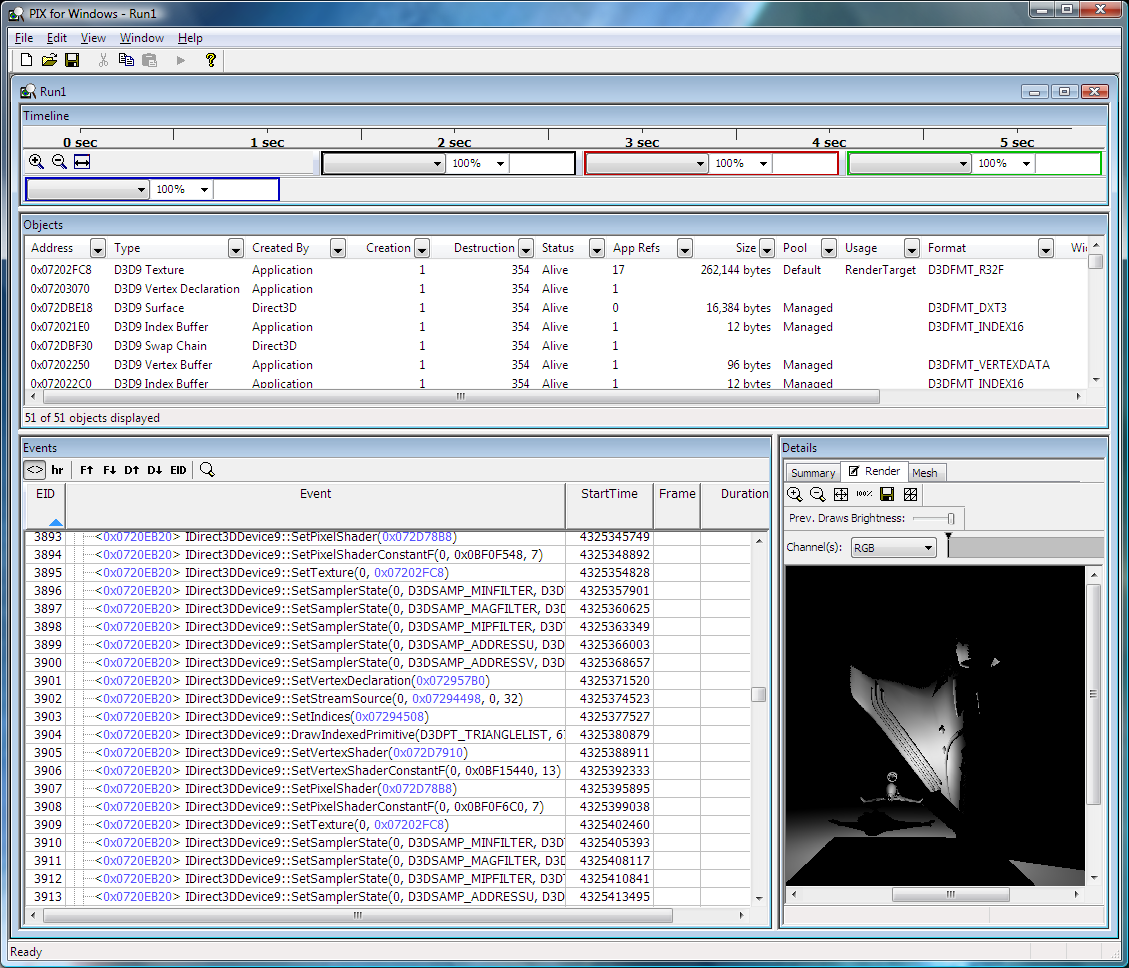
\includegraphics[scale=0.38]{images/PIX.png}
%\caption{Debuggen von Direct3D Anwendungen mit Microsofts  PIX for Windows}\label{fig:pix}
%\end{figure}
%	
\Horde\ hat derzeit nur einen OpenGL Renderpfad und somit ist die Verwendung von PIX f�r \Horde-Anwendungen unm�glich. Die Ziele des \DevEnvs\ unterscheiden sich allerdings haupts�chlich im Abstraktionslevel von den Zielen des Microsoft Tools: Beide Tools erlauben die Betrachtung des Zustands einer Software, die eine entsprechende API verwendet. Bei PIX ist diese API Direct3D, beim \DevEnv\ ist es \Horde. Insbesondere stammt die Idee der Funktionsaufruf-Historie und -Performanceauswertung aus PIX.
	
\subsection{NVIDIA PerfHUD}
NVIDIA PerfHUD\footnote{\url{http://developer.nvidia.com/nvperfhud_home.html}} ist ebenfalls ein Tool zum Debuggen von Direct3D-Anwendungen. Allerdings ist der Fokus nicht der gleiche wie bei PIX, sondern die Tools erg�nzen sich in ihren M�glichkeiten. So erlaubt PerfHUD ebenfalls ein schrittweises Zeichnen der Szene, unterst�tzt allerdings kein Shaderdebugging. Auch ist PerfHUD keine eigenst�ndige Anwendung wie PIX, sondern l�uft direkt in der zu debuggenden Anwendung mit. PerfHUDs Hauptaufgabe ist die Unterst�tzung der Performanceoptimierung und Auffinden von Flaschenh�lsen in der Grafik-Pipeline. Alle Performancecounter der NVIDIA Grafikkarten k�nnen mit dem Tool ausgelesen werden. Dies erm�glicht es beispielsweise, f�r einen \emph{Draw Call} die Auslastung der Shader Einheiten der Grafikkarte, die CPU-Auslastung durch den Grafikkartentreiber usw. zu ermitteln und auszuwerten.

Im Vergleich zum \DevEnv\ gibt es fast keine �berschneidungen in der Funktionalit�t. Jedoch macht es die Funktionsweise von PerfHUD erforderlich, die Szene einzufrieren. Der User Guide \cite[S. 11]{perfhud} gibt einen Hinweis darauf, dass dies technisch �ber ein "`Anhalten der Zeit"' gel�st wurde. Das \DevEnv\ verwendet einen analogen L�sungsansatz. Des Weiteren wurde Nicolas Schulz von diesem Tool inspiriert, als er den Schutz vor unerw�nschtem \emph{Reverse-Engineering} vorschlug. PerfHUD l�sst sich nur mit Anwendungen verwenden, die beim Starten ein spezielles Direct3D-\emph{Device} ausw�hlen. W�hlt die Anwendung in \emph{Release Builds} das PerfHUD-\emph{Device} nicht aus, verweigert das Tool seinen Dienst. Damit k�nnen Konkurrenzfirmen nicht herausfinden, wie die Anwendung eine Szene berechnet und auf welche Performancecharakteristika die Anwendung optimiert wurde.

\subsection{NVIDIA FxComposer und AMD RenderMonkey Toolsuite}
NVIDIA FxComposer\footnote{\url{http://developer.nvidia.com/object/fx_composer_home.html}} und AMD RenderMonkey Toolsuite\footnote{\url{http://developer.amd.com/GPU/RENDERMONKEY/Pages/default.aspx}} sind Entwicklungsumgebungen f�r Shader und Materials. Sie bieten eine Vorschau der erstellten Effekte an und k�nnen diese in verschiedene Formate f�r OpenGL- und Direct3D-Anwendungen exportieren. Allerdings gibt es derzeit keinen Exporter f�r das \Horde-Shaderformat und GLSL wird von beiden Tools nicht direkt unterst�tzt.

Im Gegensatz zum \DevEnv\ ist jedoch keine direkte Integration mit der Anwendung vorgesehen; die erstellten Shader und Materials k�nnen also nicht sofort in der Anwendung betrachtet werden. 
\section{Konklusion}
Es stellte sich als die richtige Entscheidung heraus, die Funktionsweise und den Aufbau von \Horde\ vor der eigentlichen Anforderungsanalyse genau zu untersuchen. Dadurch konnten wichtige Einblicke in den Problembereich gewonnen werden, da das Konzeptmodell fast komplett vorgegeben wurde. Zusammen mit den Erfahrungen aus der Entwicklung von SheepMeUp konnten viele Systemanforderungen gefunden werden, die sp�ter als hilfreich und wichtig best�tigt wurden.

%Das Konzeptmodell war eine gro�e Hilfe in der Design-Phase und wurde in sp�teren Iterationen fast nicht ver�ndert. Die Anforderungen an das System wurden im Design und in der Implementierung vollst�ndig umgesetzt und erwiesen sich als �u�ert hilfreich bei der Entwicklung eines Hitzeschimmer-Effekts f�r \SheepMeUp.

Die Betrachtung �hnlicher und verwandter Softwaretools best�tigte au�erdem, dass es f�r \Horde\ kein zum \DevEnv\ vergleichbares Tool gibt. Des Weiteren konnten einige Ideen der Tools in die Anforderungen, das Design oder die Implementierung des Systems integriert werden.